\documentclass[a4paper]{article}

\usepackage[english]{babel}
\usepackage[utf8]{inputenc}
\usepackage{amsmath}
\usepackage{graphicx}
\usepackage[colorinlistoftodos]{todonotes}
\usepackage{comment}
\usepackage{float}
\usepackage{placeins}
\usepackage{textcomp}

\title{MPRA Protocol}

\begin{document}
\maketitle

\newpage
\tableofcontents
\newpage

\section{Library Design}
	\subsection{Fragments} 
    	\begin{itemize}
                	
            \item Fragment size is limited by sequencing capacity. The maximum insert size is the maximum synthesis length minus 30 base pairs to account for incorporation of flanking amplification primers. 
                              
    	\end{itemize}
	
    \subsection{Library Primers} 
    	\begin{itemize}
            
            \item First set of primers are un-tailed \\
            Forward: 5' - GCCAGAACATTTCTCT - 3'\\
            Reverse:   5' - GCAGGAGCCGCAGTG - 3'
           
            \item Second set primers utilize tails to add restriction sites and tags to synthesized fragments.
            
            \item The Forward primer adds SwiI (GGCCNNNNNGGCC) cloning site:\\\\
            5' - GCCAGAACATTTCTCT\textbf{GGCCTAACTGGCC}GCTTGACG - 3'
           \item The Reverse primer adds SwiI (GGCCNNNNNGGCC), KpnI(CCATGG), XbaI(AGATCT), and a 16bp tag sequence:\\

				\begin{table}[h]
                    \centering
 					\begin{tabular}{c}
									 	\tiny{CCGACTAGCTT\textbf{GGCCGCCGAGGCC}CGACGCTCTTCCGATCTNNNNNNNNNNNNNNNN\textbf{TCTAGA}\textbf{GGTACC}GCAGGAGCCGCAGTG}          
        			\end{tabular}  
       			 \end{table}
   
		   \item \normalsize{The Reverse primer tag sequences are made by IDT and each \textbf{N} base pair is hand mixed with all nucleotides having an equal proportion of incorporation. The resulting Primer library is purified via HPLC (PAGE has low yield and could skew representation, standard desalting would allow truncated primer products to contaminate primer pool).}

    	\end{itemize}	

\section{Library QC and Preliminary Amplification}    
    \subsection{Single Reaction} 
    	\begin{itemize}
                	
            \item \textbf{Small Cycle qPCR Library Amplification}
          
            \item Observe library amplification with flourescent SYBR Green qPCR reporting on every cycle
            \end{itemize}
        
        	\begin{figure}[H]
				\centering
				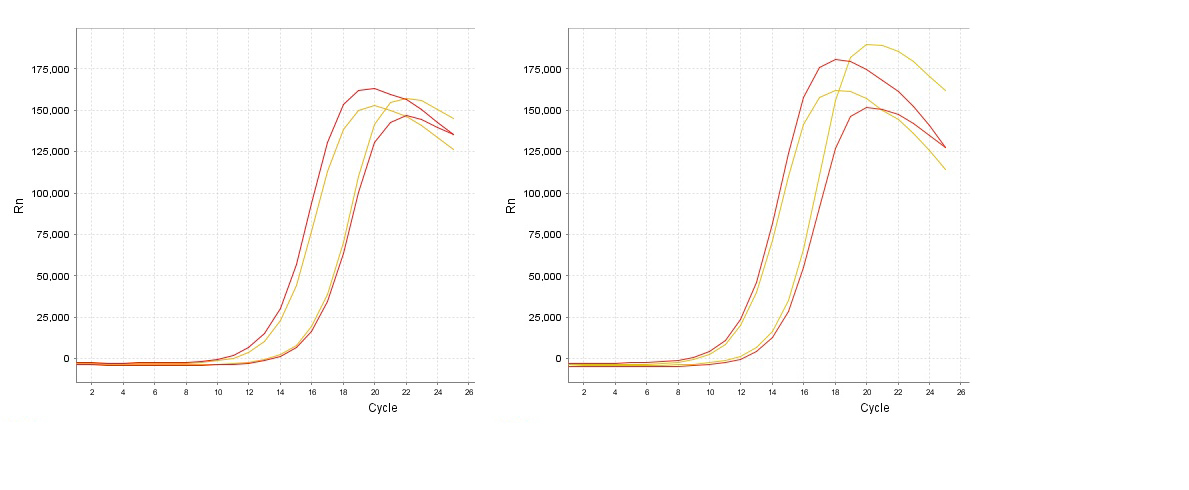
\includegraphics[width=1.0\textwidth]{2016_04_19_PremlimAMPs.jpg}
				\label{fig:Initial qPCR Library Amplification}
				\caption{Initial qPCR Library Amplification Left: Human, Right: Chimp}
		
        	\end{figure}
        	\begin{itemize}

			\item \textbf{PCR Mix:}
          \end{itemize}
         \FloatBarrier
         \begin{table}[H]
			\centering
			\begin{tabular}{l|r|r}
					Reagent 									& 	Volume 				& 	30x 		\\\hline
					2x NEB Master Mix 							& 	10\textmu L 		& 	300\textmu L		\\
					Water 										& 	6.55\textmu L		& 	196.5\textmu L		\\
                    Fwd + Rev Primers (10\textmu mol/\textmu L)	& 	1.25\textmu L		& 	37.5\textmu L		\\
                    10x SYBR Green 								& 	1.2\textmu L		& 	-\textmu L			\\
                    DNA 1:10 dilution							& 	1\textmu L			& 	-\textmu L	\\\hline
                    Final Volume 								& 	20\textmu L			& 	600\textmu L		\\
				\end{tabular}
           		\caption{\label{qPCR}Initial Library PCR.}
        \end{table}     
        \begin{itemize}
			
            \item Pipette out 17.8\textmu L into 7 wells on qPCR plate. 
        	
            \item Add SYBR green and DNA to 5 wells (Fluorescent Reporter Wells)
           	
            \item Add SYBR green and Water in place of DNA to 2 wells (Control Wells)

			\item Add water instead of SYBR green and and DNA to the 23 reaction Master Mix
            
        	\item Pipette 20 wells to collect for purification 

           	\item \textbf{PCR Conditions:}
            	\end{itemize}
         \FloatBarrier
         \begin{table}[H]
			\centering
			\begin{tabular}{l|r|r|l|r}
				Stage 	& 	Temperature	&	Time	&	Cycles		\\\hline
				Stage 1	&	98C			&	30 Sec	&	1 Cycle		\\\hline
						&	98C			&	10 Sec.	&				\\
                Stage 2	&	62C			&	30 Sec.	&	X Cycles	\\
                  		&	72C			&	30 Sec.	&				\\\hline
                Stage 3	&	72C			&	5 Min.	&	1 Cycle		\\
				\end{tabular}
           		\caption{\label{LibqPCRPCR}qPCR Amplification Conditions.}
          \end{table}
            
        \begin{itemize}
        	
            \item Amplification cycles are determined empirically to stop amplification in the log phase
        
        \end{itemize}
        
        	\begin{figure}[H]
				\centering
				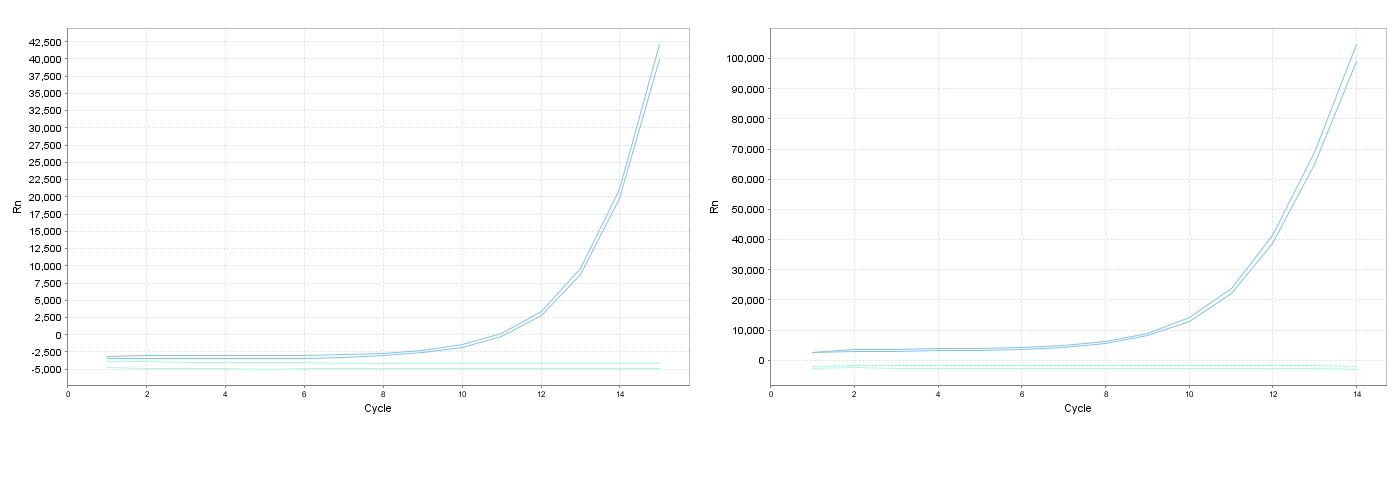
\includegraphics[width=1.0\textwidth]{2016_04_21_Scaled_LibAmp.jpg}
				\label{fig:Scaled qPCR Library Amplification}
				\caption{Left: Human, Right: Chimp}
		
        	\end{figure}
        \begin{itemize}
        
        \item Bead Purified 2x Volume ratio. Elute in 50\textmu L qiagen EB
        
        \end{itemize}
        
\section{Emulsion PCR (CHIMERx: 3600-02)} 
	\subsection{Reaction Mix} 
    	 \begin{itemize}
                	
            \item \textbf{Emulsion:}
          \end{itemize}
         \FloatBarrier
         \begin{table}[H]
			\centering
			\begin{tabular}{l|r|r}
					Reagent 				&	Volume	&	16x 			\\\hline
					Emulsion Component 1 	& 	220		&	3520\textmu L 	\\
					Emulsion Component 3 	& 	60		&	960\textmu L	\\
                    Emulsion Component 2 	& 	20		&	320\textmu L	\\\hline
                    Final Volume & 300\textmu L
				\end{tabular}
           		\caption{\label{Emulsion}Emulsion Component Mixture.}
        \end{table}     
        \begin{itemize}
			
            \item Add components in order, use a wide bore tip for Emulsion Component 2.

            \item Incubate at 4C for 30 minutes on wet ice.
            
            \item \textbf{Aqueous PCR Mix:}
          \end{itemize}
         \FloatBarrier
         \begin{table}[H]
			\centering
			\begin{tabular}{l|r|r}
					Reagent 									& 	Volume 			& 	16x 			\\\hline
					2x NEB Master Mix 							& 	25\textmu L 	& 	400\textmu L		\\
					Water 										& 	19\textmu L		& 	304\textmu L		\\
                    Fwd + Rev Primers (10\textmu mol/\textmu L)	& 	2.5\textmu L	& 	40\textmu L	\\
                    BSA(10mg/mL) 								& 	2\textmu L		& 	32\textmu L		\\
                    DNA 										& 	1\textmu L		& 	16\textmu L		\\
                    q5 Pol 										& 	0.5\textmu L	& 	8\textmu L	\\\hline
                    Final Volume 								& 	50\textmu L		& 	800\textmu L	\\
				\end{tabular}
           		\caption{\label{Emulsion}Emulsion Component Mixture.}
        \end{table}     
        \begin{itemize}
			
            \item Add entire volume to pre-chilled emulsion mix and vortex for 5 minutes on high at 4C.
        	
            \item \textbf{PCR Conditions:}
            
         \end{itemize}
         \FloatBarrier
         \begin{table}[H]
			\centering
			\begin{tabular}{l|r|r|l|r}
				Stage 	& 	Temperature	&	Time	&	Cycles		\\\hline
				Stage 1	&	98C			&	30 Sec	&	1 Cycle		\\\hline
						&	98C			&	20 Sec.	&				\\
                Stage 2	&	72C			&	10 Sec.	&	15 Cycles	\\
                  		&	72C			&	15 Sec.	&				\\\hline
                Stage 3	&	72C			&	5 Min.	&	1 Cycle		\\
				\end{tabular}
           		\caption{\label{LibPCR}PCR Conditions for Library Insert Amplification.}
          \end{table}
            
        \begin{itemize}
        
			\item Each PCR reaction is 50\textmu L per-well.
        	
            \item \textbf{Cleanup:}
            
            \item Pool all reactions and add 1mL of 2-butanol. Vortex thoroughly.
            
            \item Use kit provided spin columns

        \end{itemize}
        
      \subsection{Full Scale Reaction} 
    	 \begin{itemize}
                	
            \item \textbf{Emulsion:}
          \end{itemize}
         \FloatBarrier
         \begin{table}[H]
			\centering
			\begin{tabular}{l|r}
					Reagent & Volume \\\hline
					Emulsion Component 1 & 3520\textmu L \\
					Emulsion Component 3 & 960\textmu L\\
                    Emulsion Component 2 & 320\textmu L\\\hline
                    Final Volume & 300\textmu L
				\end{tabular}
           		\caption{\label{Emulsion}Emulsion Component Mixture.}
        \end{table}     
        \begin{itemize}
			
            \item Add components in order, use a wide bore tip for Emulsion Component 2.

            \item Incubate at 4C for 30 minutes on wet ice.
            
            \item \textbf{Aqueous PCR Mix:}
          \end{itemize}
         \FloatBarrier
         \begin{table}[H]
			\centering
			\begin{tabular}{l|r}
					Reagent 									& 	Volume 			\\\hline
					2x NEB Master Mix 							& 	400\textmu L 	\\
					Water 										& 	319\textmu L		\\
                    Fwd + Rev Primers (10\textmu mol/\textmu L)	& 	40\textmu L	\\
                    BSA(10mg/mL) 								& 	32\textmu L		\\
                    DNA 										& 	1\textmu L		\\
                    q5 Pol 										& 	8\textmu L	\\\hline
                    Final Volume 								& 	800\textmu L
				\end{tabular}
           		\caption{\label{Emulsion}Emulsion Component Mixture.}
        \end{table}     
        \begin{itemize}
			
            \item Add entire volume to pre-chilled emulsion mix and vortex for 5 minutes on high at 4C.
        	
            \item \textbf{PCR Conditions:}
            
         \end{itemize}
         \FloatBarrier
         \begin{table}[H]
			\centering
			\begin{tabular}{l|r|r|l|r}
				Stage 	& 	Temperature	&	Time	&	Cycles		\\\hline
				Stage 1	&	98C			&	30 Sec	&	1 Cycle		\\\hline
						&	98C			&	20 Sec.	&				\\
                Stage 2	&	72C			&	10 Sec.	&	15 Cycles	\\
                  		&	72C			&	15 Sec.	&				\\\hline
                Stage 3	&	72C			&	5Min.	&	1 Cycle		\\
				\end{tabular}
           		\caption{\label{LibPCR}PCR Conditions for Library Insert Amplification.}
          \end{table}
            
        \begin{itemize}
        
			\item Each PCR reaction is 50\textmu L per-well (96 wells total).
        	
            \item \textbf{Cleanup:}
            
            \item Pool all reactions and add 13.7mL of 2-butanol. Vortex thoroughly.
            
            \item Use kit provided spin columns. Condense all volume over 3-4 columns to concentrate eluted library

        \end{itemize}
	
    \subsection{Size Select Library to Remove Slippage Products} 
      	\begin{itemize}
    		\item Slippage on the the random tag sequence causes the production of additional products to arise from the emulsion PCR
        
        \end{itemize}
        
        	\begin{figure}[H]
				\centering
				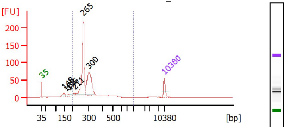
\includegraphics[width=1.0\textwidth]{EmulsionPCRIssue.jpg}
				\label{fig:Bioanalyzer trace}
				\caption{Extra large molecular weight slippage product ~300bp}
        	\end{figure}
        \begin{itemize}
    	
        	\item Foo
        
        \end{itemize}
\section{Library Cloning}    
    
\section{Library Sequencing}    

\section{Library Transfection}    

\section{Post Transfection Processing}    


\section{Reagents}
    
\section{Primer Sequences}

%\begin{enumerate}
%\item Like this,
%\item and like this.
%\end{enumerate}
%\dots or bullet points \dots
%\begin{itemize}
%\item Like this,
%\item and like this.
%\end{itemize}
%\dots or with words and descriptions \dots
%\begin{description}
%\item[Word] Definition
%\item[Concept] Explanation
%\item[Idea] Text
%\end{description}


\end{document}